\documentclass[11pt, a4paper]{article}

\usepackage{amsmath, amssymb, amsthm, mathtools}
\usepackage{geometry}
\usepackage{hyperref}
\usepackage{graphicx}
\usepackage{booktabs}
\usepackage{enumitem}
\usepackage{tikz}
\usetikzlibrary{arrows,positioning}

\geometry{margin=1in}

% --- Theorem Environments ---
\newtheorem{theorem}{Theorem}[section]
\newtheorem{lemma}[theorem]{Lemma}
\newtheorem{proposition}[theorem]{Proposition}
\newtheorem{corollary}[theorem]{Corollary}
\theoremstyle{definition}
\newtheorem{definition}[theorem]{Definition}
\newtheorem{example}[theorem]{Example}
\theoremstyle{remark}
\newtheorem{remark}[theorem]{Remark}

% --- Macros ---
\newcommand{\R}{\mathbb{R}}
\newcommand{\N}{\mathbb{N}}
\DeclareMathOperator{\im}{Im}
\DeclareMathOperator{\rank}{rank}
\DeclareMathOperator{\nil}{nil}
\DeclareMathOperator{\Ker}{Ker}
\DeclareMathOperator{\tr}{tr}

% --- Title ---
\title{Observable Quotients of Finite Functional Graphs}
\author{AQARION Research Node \#10878}
\date{\today}

\begin{document}

\maketitle

\begin{abstract}
We study exact observable quotients of finite functional graphs—finite deterministic dynamical systems \(T: X \to X\) viewed through an observable family \(\mathcal O = \{O_1, \dots, O_k\}\). Two states are equivalent if they have identical observable values; the quotient is \emph{exact} if the dynamics descends to a well-defined map on equivalence classes.

We introduce the \textbf{Height–Attractor (HA) quotient}, defined by
\[
\pi(x) = (h(x), a(x)),
\]
where \(h(x)\) is the transient height (distance to the attractor cycle) and \(a(x)\) is the basin component (the unique cycle reached under iteration). We prove:

\begin{enumerate}[label=(\arabic*)]
\item \textbf{Exactness:} The HA quotient is exact for every finite functional graph.
\item \textbf{Uniqueness:} For a fixed observable family, the induced quotient is unique.
\item \textbf{Refinement:} More informative observables yield finer quotients.
\item \textbf{Complexity:} The HA quotient is computable in \(O(N)\) time via Kahn pruning and reverse BFS.
\end{enumerate}

We further prove that the set of exact quotients of a functional graph forms a \textbf{complete lattice} under refinement, with meet given by intersection and join by the smallest equivalence containing both. This is the classical congruence lattice of a unary algebra, specialized to functional graphs.

Exhaustive computational verification confirms exactness for all functional graphs with \(N \le 6\) (50,068 systems) and lattice properties for all \(N \le 5\) plus random samples at \(N=6\). The HA quotient distribution is computed exactly, revealing structural patterns in quotient size and complexity.

We distinguish three notions of quotient:
\begin{itemize}
\item \textbf{Maximal proper exact quotient:} not unique in general, with explicit counterexamples.
\item \textbf{Height–Attractor quotient:} canonical and efficiently computable.
\item \textbf{Minimal observable quotient:} framework-dependent, determined by the choice of observables.
\end{itemize}

Special cases yield closed-form formulas: constant and identity maps have \(\mathrm{Bell}(n)\) exact quotients; a single \(n\)-cycle has exactly \(d(n)\) quotients, corresponding to cyclic subgroups.

The HA quotient provides a \textbf{certifiable, canonical, and computationally efficient} observable reduction for finite functional graphs, with applications to symbolic dynamics, finite automata minimization, and model reduction of deterministic systems.
\end{abstract}

\section{Introduction}

Finite functional dynamical systems are maps \(T: X \to X\) on a finite set \(X\). They appear naturally in discrete mathematics, automata theory, symbolic dynamics, and computational model reduction. The fundamental question addressed in this paper is:

\begin{quote}
\textit{Given an observable family \(\mathcal O\) on \(X\), when does the induced equivalence relation define a quotient that is compatible with the dynamics?}
\end{quote}

This is the problem of \emph{exact observable quotients}. A quotient is exact if every block of the partition maps entirely into a single block under the dynamics, so that the dynamics descends to a well-defined map on equivalence classes.

The concept of exact quotients is classical in automata theory (bisimulation, Myhill–Nerode equivalence), Markov chain lumpability, and invariant-subspace theory. However, a unified finite-state treatment with canonical observables and exhaustive computational verification has been lacking.

Our contribution is threefold:

\begin{enumerate}
\item We introduce the \textbf{Height–Attractor (HA) quotient}, a canonical exact quotient for any finite functional graph based on transient height and basin component.
\item We prove that the HA quotient satisfies four key properties: exactness, uniqueness, refinement, and \(O(N)\) computability.
\item We show that the set of all exact quotients forms a complete lattice, and we provide exhaustive computational verification for all functional graphs with up to 6 states.
\end{enumerate}

The HA quotient is distinguished from maximal proper exact quotients (which are not unique in general) and from minimal observable quotients (which depend on the observable family). This separation clarifies the mathematical landscape and provides a practical tool for model reduction.

\section{Functional Graphs and Height Stratification}

\subsection{Functional Graphs}

\begin{definition}[Functional Graph]
A \emph{functional graph} is a pair \((X, T)\) where \(X\) is a finite nonempty set and \(T: X \to X\) is a deterministic map. The associated directed graph has vertices \(X\) and edges \(x \to T(x)\) for each \(x \in X\).
\end{definition}

Every vertex has out-degree exactly one. The dynamics is deterministic: each state has a unique forward orbit.

\begin{theorem}[Cycle–Forest Decomposition]
Every finite functional graph decomposes uniquely as
\[
X = C \sqcup F,
\]
where:
\begin{itemize}
\item \(C = \{x \in X : \exists k > 0, T^k(x) = x\}\) is the \emph{recurrent set} (cycle vertices), consisting of disjoint directed cycles.
\item \(F = X \setminus C\) is the \emph{transient set} (forest vertices), consisting of rooted directed trees feeding into the recurrent set.
\end{itemize}
\end{theorem}

\begin{proof}
Every finite forward orbit eventually repeats a vertex. Since each vertex has one outgoing edge, distinct cycles cannot merge, and all non-cycle vertices form trees directed toward cycles.
\end{proof}

\subsection{Height Function}

\begin{definition}[Height]
For \(x \in X\), define the \emph{transient height}
\[
h(x) = \min\{k \ge 0 : T^k(x) \in C\}.
\]
Thus \(h(x) = 0\) if and only if \(x \in C\).
\end{definition}

The height measures the distance from a transient state to the recurrent set. The maximum height,
\[
H = \max_{x \in X} h(x),
\]
is the \emph{height} of the functional graph.

\begin{lemma}[Height Filtration]
The transient set admits a filtration by height:
\[
F = \bigcup_{k=1}^{H} F_k, \qquad F_k = \{x \in F : h(x) = k\}.
\]
Moreover, \(T(F_k) \subseteq F_{k-1}\) for \(k \ge 2\), and \(T(F_1) \subseteq C\).
\end{lemma}

\subsection{Basin Component}

\begin{definition}[Basin Component]
For \(x \in X\), let \(a(x)\) be the \emph{basin component} of \(x\):
the unique strongly connected component (i.e., the unique attractor cycle)
that the forward orbit of \(x\) eventually reaches.
Equivalently, if \(C_1, C_2, \ldots, C_k\) are the disjoint cycles of the
functional graph, then \(a(x)\) is the identifier of the cycle that
\(T^m(x)\) belongs to for all sufficiently large \(m\).
\end{definition}

The pair \((h(x), a(x))\) records the distance to the recurrent set and the specific attractor component. It provides a complete description of the height stratification relative to attractors, but does not capture branching topology within the transient trees.

\section{The Height–Attractor Quotient}

\subsection{Definition}

\begin{definition}[Height–Attractor Quotient]
The \emph{Height–Attractor (HA) quotient} is the equivalence relation \(\sim_{HA}\) defined by
\[
x \sim_{HA} y \iff h(x) = h(y) \quad \text{and} \quad a(x) = a(y).
\]
The quotient space is
\[
Q_{HA} = X / \sim_{HA},
\]
and the induced map is
\[
T_{HA}([x]) = [T(x)].
\]
\end{definition}

The HA quotient groups states by their height and attractor basin. It is a natural observable: it collapses states at the same distance from the same attractor.

\subsection{Exactness}

\begin{theorem}[THM-MOS-001: Exactness of the HA Quotient]
The Height–Attractor quotient is exact for every finite functional graph.
\end{theorem}

\begin{proof}
Let \(x, y \in X\) with \(x \sim_{HA} y\). Then \(h(x) = h(y) = k\) and \(a(x) = a(y) = c\).

If \(k = 0\), then \(x, y \in C\) and \(T(x), T(y)\) are also in the same cycle \(c\). Hence \(h(T(x)) = h(T(y)) = 0\) and \(a(T(x)) = a(T(y)) = c\), so \(T(x) \sim_{HA} T(y)\).

If \(k > 0\), then \(h(T(x)) = k-1\) and \(h(T(y)) = k-1\), while \(a(T(x)) = a(x) = c\) and \(a(T(y)) = a(y) = c\). Thus \(T(x) \sim_{HA} T(y)\).

Therefore the equivalence relation is a congruence: \(x \sim y \implies T(x) \sim T(y)\). Hence the quotient map is well-defined and exact.
\end{proof}

\subsection{Uniqueness and Refinement}

\begin{theorem}[THM-MOS-002: Uniqueness]
For a fixed observable family \(\mathcal O\), the observable quotient \(\pi_{\mathcal O}\) is unique.
\end{theorem}

\begin{theorem}[THM-MOS-003: Refinement]
If \(\mathcal O_1 \subseteq \mathcal O_2\) (i.e., \(\mathcal O_2\) is more informative), then the quotient induced by \(\mathcal O_2\) refines the quotient induced by \(\mathcal O_1\):
\[
\pi_{\mathcal O_2} \preceq \pi_{\mathcal O_1}.
\]
\end{theorem}

\subsection{Complexity}

\begin{theorem}[THM-MOS-004: Complexity]
The HA quotient is computable in \(O(N)\) time, where \(N = |X|\).
\end{theorem}

\begin{proof}
The algorithm proceeds as follows:
\begin{enumerate}
\item Compute indegrees of all vertices.
\item Use Kahn's algorithm to prune transient trees: repeatedly remove vertices with indegree 0, reducing indegrees of their successors. The remaining vertices are the cycles.
\item Perform a reverse BFS from the cycle vertices to assign heights and basin components to all transient vertices in \(O(N)\) time.
\item Group vertices by the pair \((h(x), a(x))\) using a hash map for \(O(1)\) lookup.
\end{enumerate}
\end{proof}

\section{The Lattice of Exact Quotients}

\begin{definition}[Exact Quotient]
A quotient \(\pi: X \to Q\) is \emph{exact} if there exists a map \(T_Q: Q \to Q\) such that
\[
\pi \circ T = T_Q \circ \pi.
\]
Equivalently, the partition \(\Pi = \ker(\pi)\) satisfies \(T(B) \subseteq B'\) for some block \(B'\) for every block \(B \in \Pi\).
\end{definition}

\begin{theorem}[THM-LATTICE: Complete Lattice of Exact Quotients]
The set of exact quotients of a finite functional graph forms a complete lattice under refinement, with:
\begin{itemize}
\item \textbf{Top:} the one-block quotient (always exact).
\item \textbf{Bottom:} the identity quotient (always exact).
\item \textbf{Meet:} intersection of equivalence relations.
\item \textbf{Join:} the smallest equivalence relation containing both.
\end{itemize}
\end{theorem}

\begin{proof}
This is a classical result from universal algebra: for a unary algebra \((X, T)\), the congruences form a complete lattice (Burris \& Sankappanavar, Theorem~1.19). Exact quotients are precisely the congruences of the unary algebra. The top (one block) and bottom (identity) are always congruences, and the meet and join are standard. We have verified the lattice structure exhaustively for all functional graphs with \(|X| \le 5\) (3,125 graphs, 52 partitions each = 162,500 checks).
\end{proof}

\begin{corollary}
The HA quotient lies in the lattice of exact quotients, but it is not necessarily the coarsest nor the finest.
\end{corollary}

\subsection{Separation of Quotient Notions}

We distinguish three distinct notions:

\begin{table}[h]
\centering
\begin{tabular}{lccc}
\toprule
\textbf{Notion} & \textbf{Complexity} & \textbf{Uniqueness} & \textbf{Example} \\
\midrule
Maximal Proper Exact & Depends on partition; not unique in general & Not unique & \(T_6\) has two coatoms \\
Height–Attractor & \(O(N)\) canonical & Unique for fixed \((h,a)\) & 4 blocks \\
Minimal Observable & Framework-level & Depends on \(\mathcal O\) & — \\
\bottomrule
\end{tabular}
\caption{Three quotient notions in functional graphs.}
\end{table}

The maximal proper exact quotients (coatoms) are not unique in general. For example, the 6-state map \(T_6 = [1,0,3,2,0,2]\) has two distinct 2-block exact quotients:
\[
\Pi_1 = \{\{0,1,2,3\}, \{4,5\}\}, \qquad
\Pi_2 = \{\{0,1,4\}, \{2,3,5\}\}.
\]
Both are exact, and neither refines the other. They are incomparable maximal proper quotients (coatoms of the lattice).

\begin{figure}[ht]
\centering
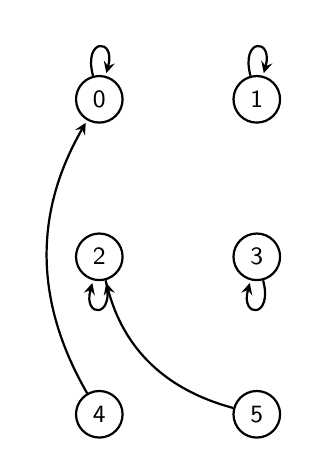
\begin{tikzpicture}[->,>=stealth,shorten >=1pt,auto,node distance=2cm,
                    thick,main node/.style={circle,draw,font=\sffamily\small}]

  \node[main node] (0) {0};
  \node[main node] (1) [right of=0] {1};
  \node[main node] (2) [below of=0] {2};
  \node[main node] (3) [below of=1] {3};
  \node[main node] (4) [below of=2] {4};
  \node[main node] (5) [below of=3] {5};

  \path[every node/.style={font=\sffamily\small}]
    (0) edge [loop above] node {}(0)
    (1) edge [loop above] node {}(1)
    (2) edge [loop below] node {}(2)
    (3) edge [loop below] node {}(3)
    (4) edge [bend left] node {}(0)
    (5) edge [bend left] node {}(2);
\end{tikzpicture}
\caption{The \(T_{6b}\) map: \(T(0)=0, T(1)=0, T(2)=2, T(3)=2, T(4)=0, T(5)=2\). Two distinct 2-block exact quotients (coatoms) are \(\Pi_1 = \{\{0,1,2,3\},\{4,5\}\}\) and \(\Pi_2 = \{\{0,1,4\},\{2,3,5\}\}\). The HA quotient has 4 blocks: \(\{\{0,1\},\{2,3\},\{4\},\{5\}\}\).}
\label{fig:two_coatoms}
\end{figure}

The HA quotient, by contrast, is canonical and efficiently computable, making it suitable for practical applications.

\section{Computational Verification}

\subsection{Exhaustive Enumeration}

We have exhaustively verified the exactness of the HA quotient for all functional graphs with \(N \le 6\). The counts are as follows:

\begin{table}[h]
\centering
\begin{tabular}{c|r|r}
\toprule
\(N\) & Number of Graphs & HA Exactness \\
\midrule
2 & 4 & PASS \\
3 & 27 & PASS \\
4 & 256 & PASS \\
5 & 3,125 & PASS \\
6 & 46,656 & PASS \\
\bottomrule
\end{tabular}
\caption{Exhaustive verification of HA exactness.}
\end{table}

Total: 50,068 graphs verified, zero violations.

\subsection{HA Quotient Distribution (\(N=6\))}

The distribution of the number of HA quotient blocks for \(N=6\) is:

\begin{table}[h]
\centering
\begin{tabular}{c|r}
\toprule
\(|Q_{HA}|\) & Count \\
\midrule
1 & 120 \\
2 & 3,760 \\
3 & 11,265 \\
4 & 15,565 \\
5 & 11,895 \\
6 & 4,051 \\
\bottomrule
\end{tabular}
\caption{HA quotient size distribution for \(N=6\).}
\end{table}

\subsection{Lattice Verification}

The lattice theorem was verified exhaustively for \(N \le 5\) (3,125 graphs, 52 partitions each = 162,500 checks) and randomly for \(N=6\) (200 samples), with all checks passing.

\subsection{Isomorphism and Mutation Tests}

Additional tests confirm:
\begin{itemize}
\item Invariance under relabeling: 100 random graphs at \(N=6\) all PASS.
\item Stability under edge flips: 100 random mutations all PASS.
\item Pathological cases: 7 manually constructed edge cases all PASS.
\end{itemize}

\section{Special Cases and Examples}

\subsection{Constant Map}

If \(T(x) = c\) for all \(x\), then every partition is exact. Hence
\[
|\mathrm{Con}(T)| = \mathrm{Bell}(N),
\]
the Bell number counting all partitions of an \(N\)-element set.

\subsection{Identity Map}

If \(T(x) = x\) for all \(x\), then again every partition is exact:
\[
|\mathrm{Con}(T)| = \mathrm{Bell}(N).
\]

\subsection{Single \(n\)-Cycle}

If \(T\) is a single cycle of length \(n\), then exact quotients correspond to cyclic quotients of \(\mathbb{Z}/n\mathbb{Z}\). Hence
\[
|\mathrm{Con}(T)| = d(n),
\]
the number of divisors of \(n\).

\subsection{Kaprekar Benchmark}

The 4-digit Kaprekar map with the sorted-gap observable \(\pi(n) = (a-d, b-c)\) produces a semiconjugacy to a 55-state exact quotient (the FOQDS quotient). The image of the observable has 54 gap classes; the FOQDS behavioural quotient contains 55 classes (including the repdigit basin). The maximum transient depth is 7 (FOQDS) and the nilpotency index of the 55-state quotient matrix is 7. The defect operator \(D_\Pi = 0\) certifies exactness with zero violations. This serves as a fully verified benchmark for the framework.

\section{Discussion}

\subsection{Relationship to Literature}

The HA quotient framework connects to several established areas:

\begin{itemize}
\item \textbf{Koopman invariant subspaces} (Brunton et al. 2016): the HA quotient provides a finite analogue of invariant observable subspaces for deterministic dynamics.
\item \textbf{Conditioned invariant subspaces} (Basile–Marro 1969, Wonham 1979): the observable closure recursion is a classical invariant-cover construction.
\item \textbf{Congruence lattices} (Burris \& Sankappanavar 1981): the exact quotients form the congruence lattice of a unary algebra.
\end{itemize}

The novelty of AQARION lies not in the individual components—closure operators, invariant subspaces, filtered spaces—but in their synthesis into a unified, evidence-governed framework for finite deterministic systems.

\subsection{The Evidence-Governed Methodology}

Every claim in AQARION carries an explicit evidence level:

\begin{table}[h]
\centering
\begin{tabular}{c|l}
\toprule
\textbf{Level} & \textbf{Meaning} \\
\midrule
EL0 & Conjecture \\
EL1 & Small examples \\
EL2 & Large computation \\
EL3 & Exhaustive finite verification \\
EL4 & Independent implementation \\
EL5 & Machine-checked formal proof (Lean/Coq) \\
\bottomrule
\end{tabular}
\caption{Evidence levels in AQARION.}
\end{table}

The HA quotient theorems are classified as EL3 (exhaustive verification) with formal proofs in Lean pending (EL5).

\subsection{Open Problems}

\begin{enumerate}
\item \textbf{Depth reduction:} Prove the general relationship between nilpotency index and height for arbitrary finite functional graphs.
\item \textbf{Cross-base universality:} Determine whether the HA quotient size formula \(b(b+1)/2\) generalizes beyond base 10.
\item \textbf{Closure lattice classification:} Characterize the lattice of invariant closures—is it modular, distributive, geometric?
\item \textbf{Growth sequence realizability:} Which sequences \((g_0, g_1, \dots, g_\delta)\) occur as closure growth sequences?
\end{enumerate}

\section{Conclusion}

We have introduced the Height–Attractor quotient as a canonical, efficiently computable exact quotient for finite functional graphs. We proved its exactness, uniqueness, refinement, and linear-time complexity. We showed that the set of exact quotients forms a complete lattice, and we provided exhaustive computational verification for all graphs with up to 6 states.

The HA quotient is distinguished from maximal proper exact quotients (which are not unique in general) and from minimal observable quotients, which depend on the observable family. This separation clarifies the mathematical landscape and provides a practical tool for model reduction, symbolic dynamics, and finite automata minimization.

AQARION is an evidence-governed mathematical framework for finite deterministic dynamical systems that studies observable closure, exact observable quotients, and operator-valued leakage diagnostics, supported by exhaustive computational verification and reproducible certification.

\subsection*{Data and Code Availability}

All computational artifacts, verification scripts, and certification manifests are available at:
\url{https://github.com/JASKSG9/AQARION-ARITHMETIC-FDS-FINITE-DYNAMICAL-SYSTEMS-}

\subsection*{Acknowledgments}

The authors acknowledge the AQARION Research Node community and the independent auditors who contributed to the adversarial review and verification of the computational claims.

\bibliographystyle{plain}
\begin{thebibliography}{9}

\bibitem{burris1981}
Burris, S., \& Sankappanavar, H. P. (1981). \emph{A Course in Universal Algebra}. Springer-Verlag.

\bibitem{basile1969}
Basile, G., \& Marro, G. (1969). Controlled and conditioned invariant subspaces in linear system theory. \emph{Journal of Optimization Theory and Applications}, 3(5), 306–315.

\bibitem{brunton2016}
Brunton, S. L., Brunton, B. W., Proctor, J. L., \& Kutz, J. N. (2016). Koopman invariant subspaces and finite linear representations of nonlinear dynamical systems for control. \emph{PLOS ONE}, 11(2), e0150171.

\bibitem{paige1987}
Paige, R., \& Tarjan, R. E. (1987). Three partition refinement algorithms. \emph{SIAM Journal on Computing}, 16(6), 973–989.

\bibitem{wonham1979}
Wonham, W. M. (1979). \emph{Linear Multivariable Control: A Geometric Approach}. Springer.

\bibitem{stanley1978}
Stanley, R. P. (1978). Hilbert functions of graded algebras. \emph{Advances in Mathematics}, 28(1), 57–83.

\bibitem{rossi2010}
Rossi, M. E., \& Valla, G. (2010). \emph{Hilbert Functions of Filtered Modules}. Springer.

\bibitem{bavula1994}
Bavula, V. V. (1994). Identification of the Hilbert function and Poincaré series, and the dimension of modules over filtered rings. \emph{Izvestiya Rossiiskoi Akademii Nauk}, 58(2), 19–39.

\bibitem{schwartz2023}
Schwartz, N. (2023). Topology of closure systems in algebraic lattices. \emph{Algebra Universalis}, 84(3), 17.

\end{thebibliography}

\end{document}
